\documentclass[../../Rapport RayTracer.tex]{subfiles}

\begin{document}


En appliquant le principe de la section \ref{rayTracingBase}, nous obtenons une image plate, sans aucun relief. Pour palier à cela, un modèle d'ombrage reste à implémenter. Ce sont en effet les ombres et les effets de lumière qui donnent aux images leur réalisme et leur relief. Un ombrage de Phong (imposé par le sujet) a donc été implémenté. L'ombrage de Phong consiste en l'addition de trois composantes distinctes:
\begin{itemize}
	\item {La composante ambiante. Elle permet de donner une luminosité minimale à la scène.}
	\item {La composante diffuse. Illumine d'autant plus l'objet que les rayons de lumière le frappe perpendiculairement.}
	\item {La composante spéculaire. Rend l'objet brillant en tenant compte de l'angle avec lequel les rayons de lumière rebondissent vers la caméra.}
\end{itemize}

\begin{figure}[h!]
	\adjustbox{center}{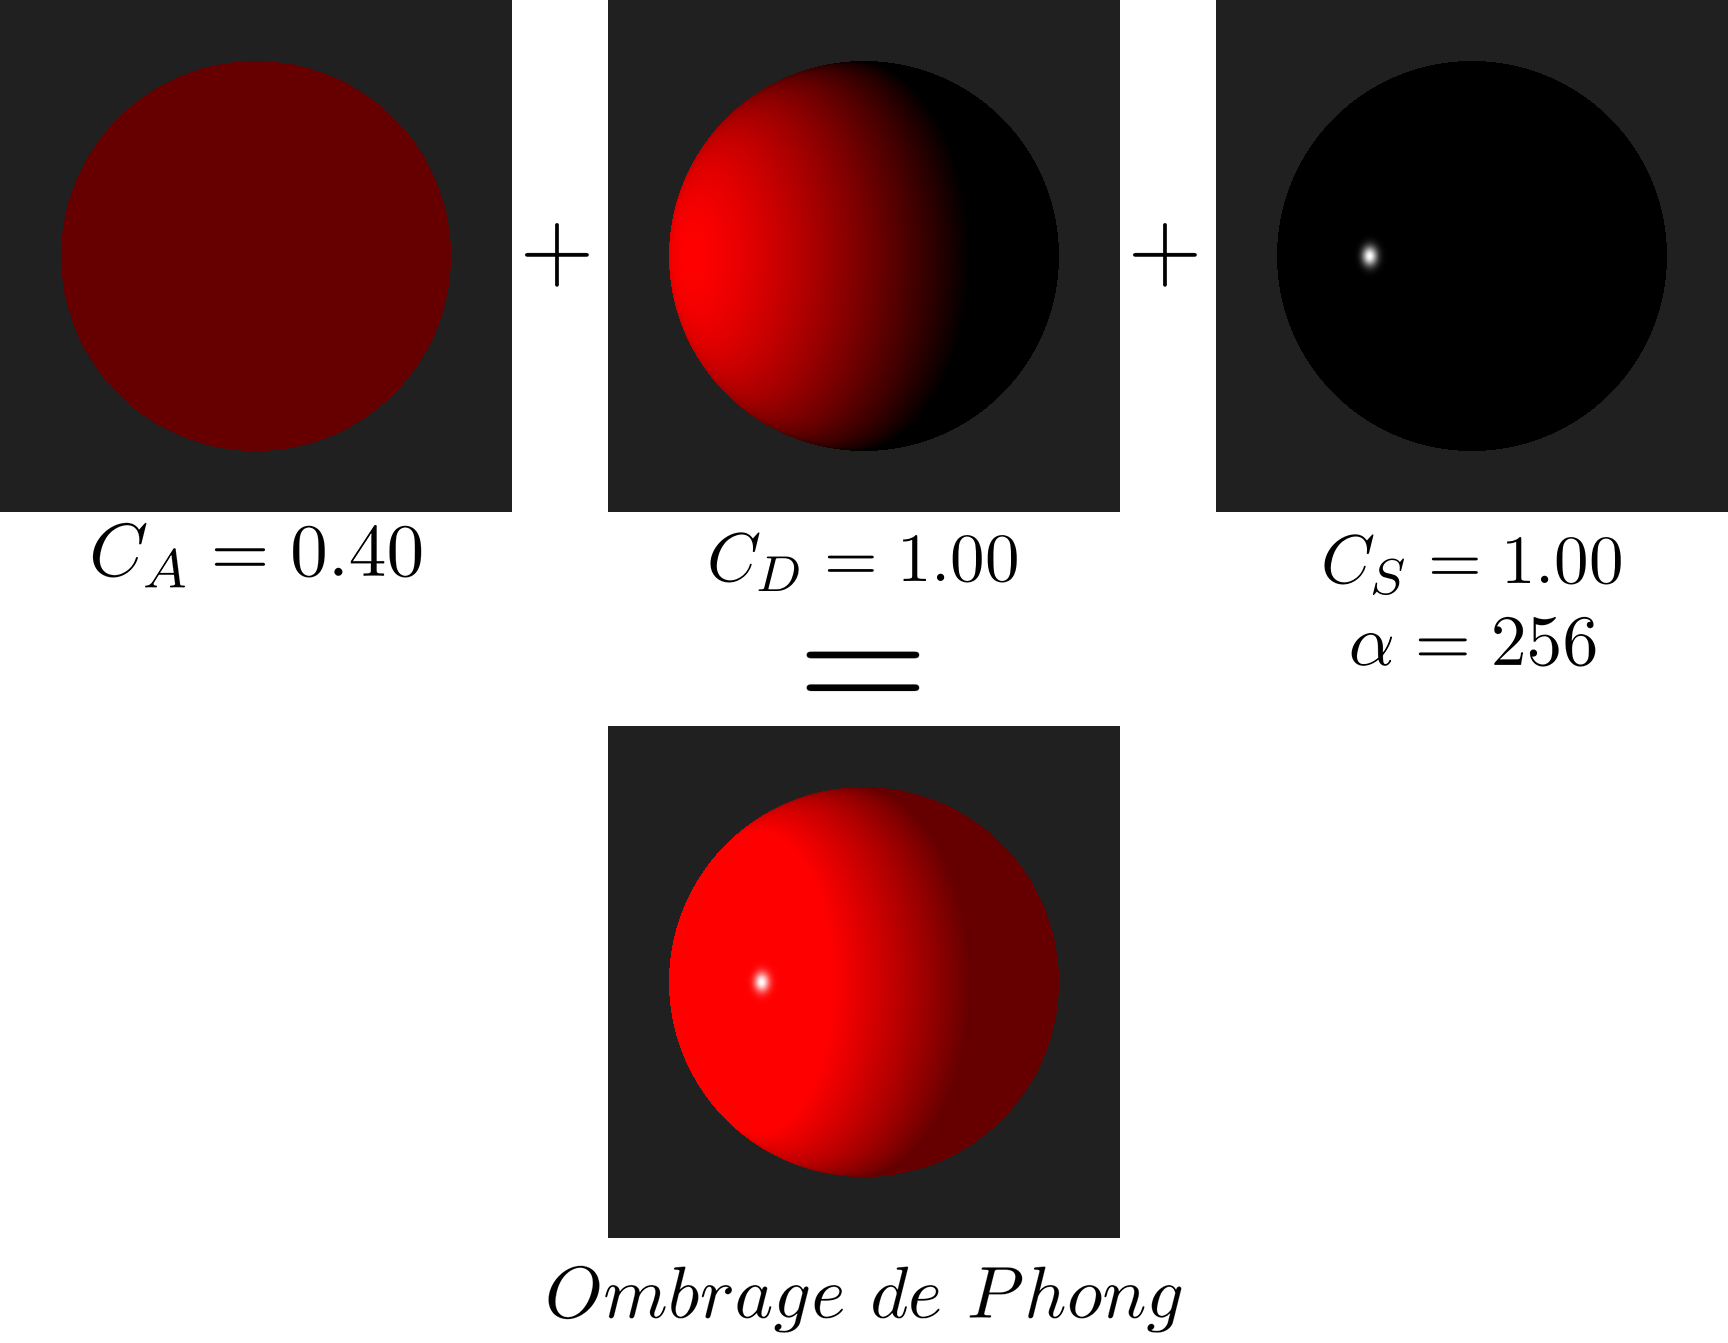
\includegraphics[width=0.75\textwidth]{img/rt/phongAddition.png}}

	\caption{Séparation des composantes de l'ombrage de Phong d'une sphère}
	\label{finalPhong}
\end{figure}
\FloatBarrier


\end{document}